\chapter{Project Design}
\section{High Level Design}
\subsection{Database Design}
    The database consists of 9 tables as described in the following ER diagram. The Prisoner table contains basic details about the the current conviction of the prisoner and the Prisoner Details table contains more descriptive details. The Work table contains details of the community service done by the prisoners. The Visitor Details table contains details of visitors visiting the various prisoners. The Cells table contains details regarding the occupants of each cell. The Staff and Login Details tables contains staff details and their login credentials respectively. The password is stored in a hashed form to enhance security.
    \begin{figure}[H]
        \centering
        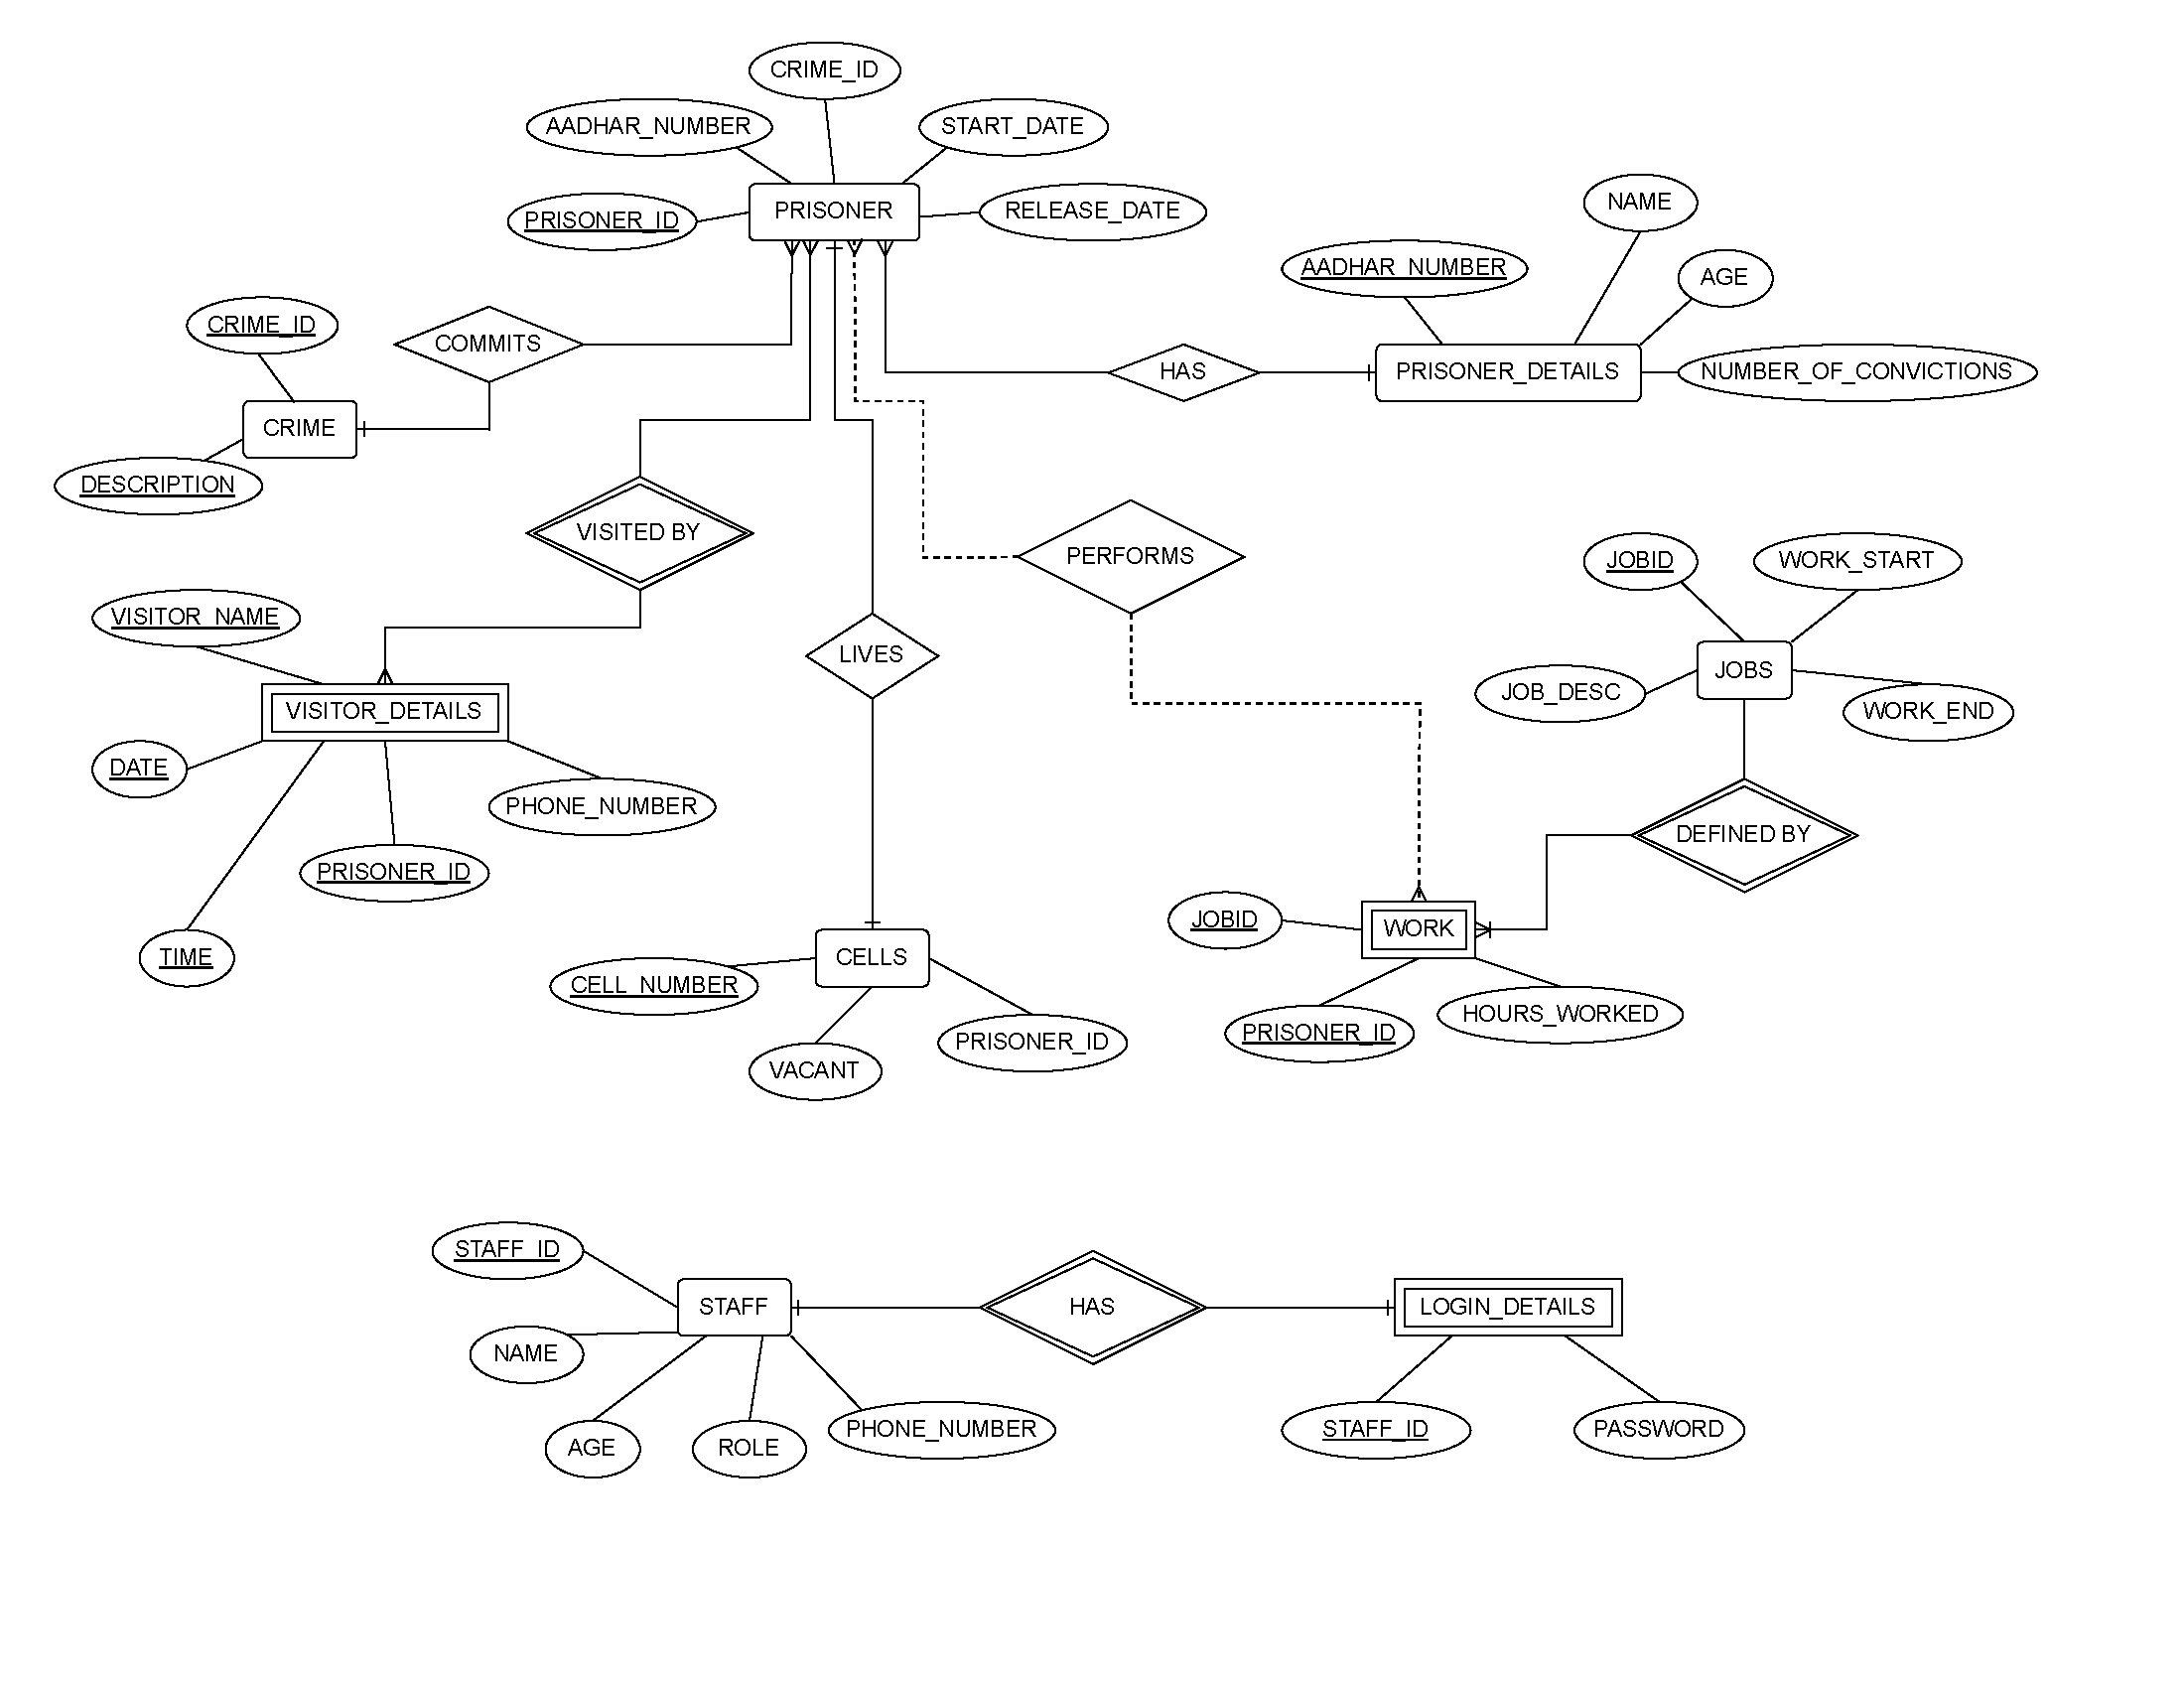
\includegraphics[ height=0.54\textheight]{er.png}
        \caption{ER Diagram}
        \label{fig:er}
    \end{figure}
\newpage
\subsection{System Design}
    The following use-case diagram is a graphical depiction of a user's possible interactions with a system. 
    \begin{figure}[H]
        \centering
        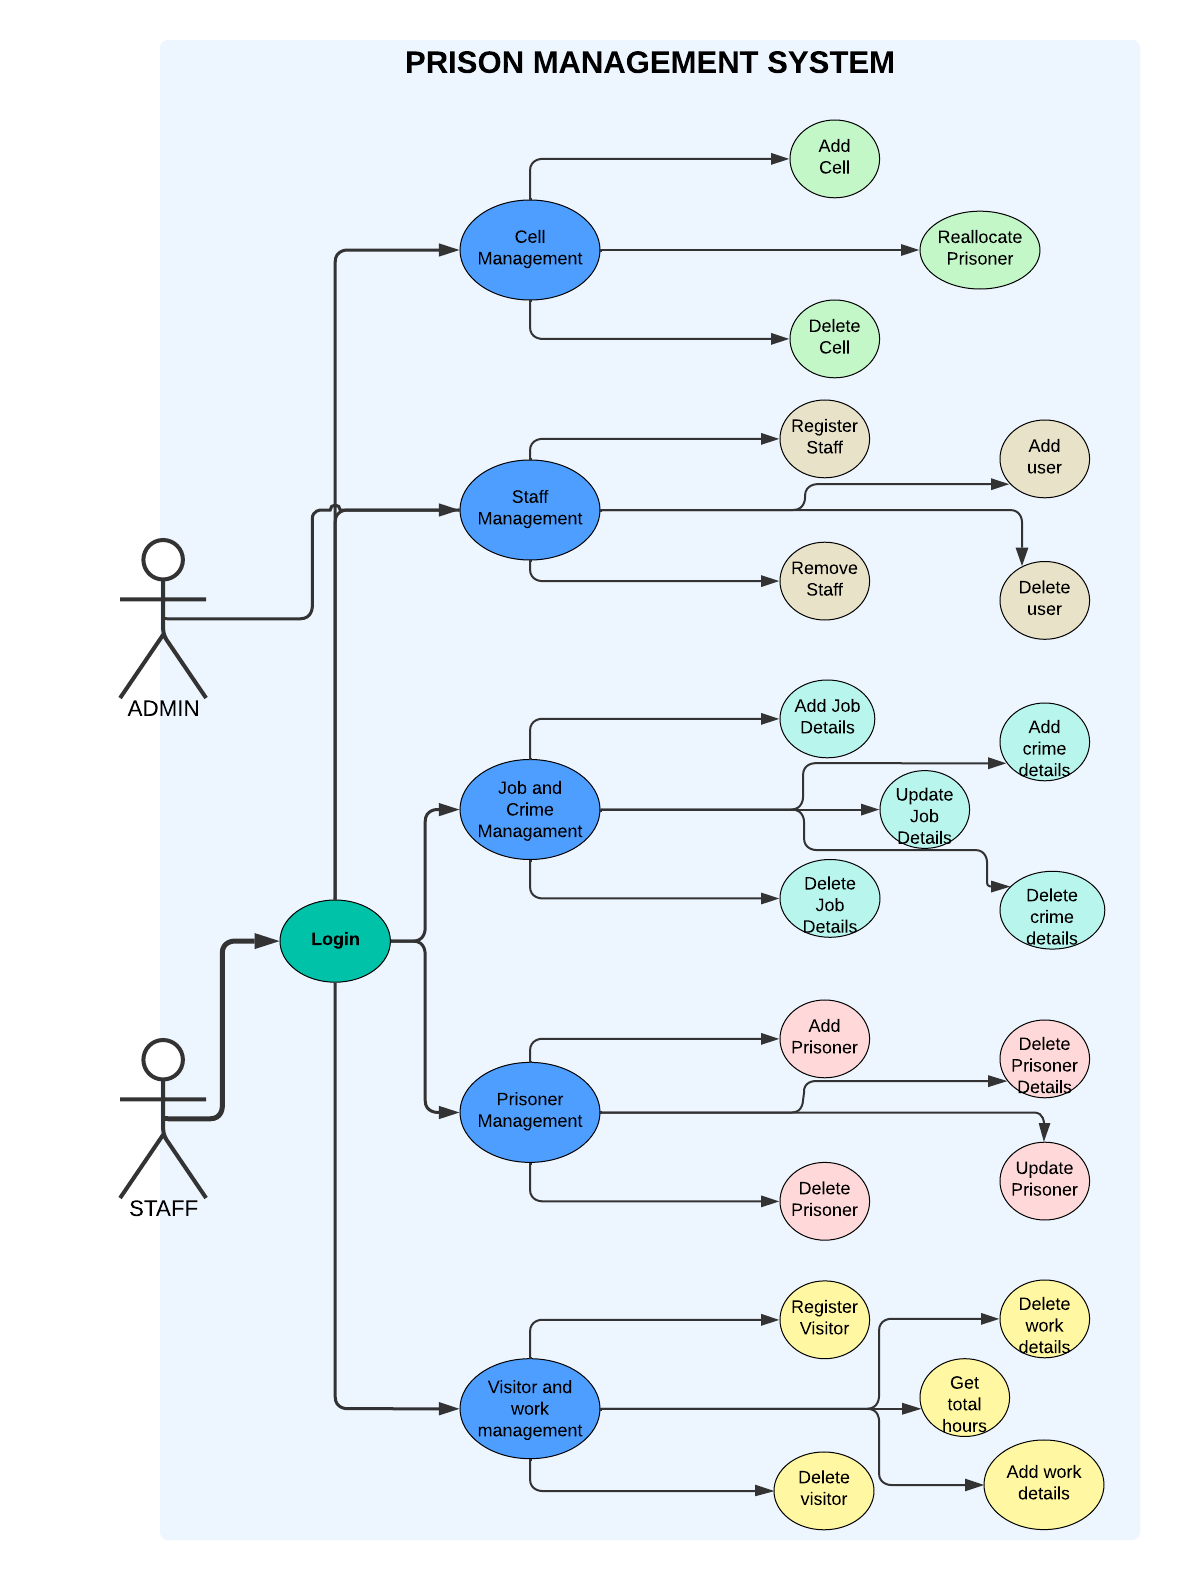
\includegraphics[width=\textwidth]{figures/use-case.png}
        \caption{Use-Case Diagram}
        \label{fig:usecase}
    \end{figure}
    \newpage
    The following class diagram shows the modularization of the system into different components. Different objects are created in order to interface with the database.
    \begin{figure}[H]
        \centering
        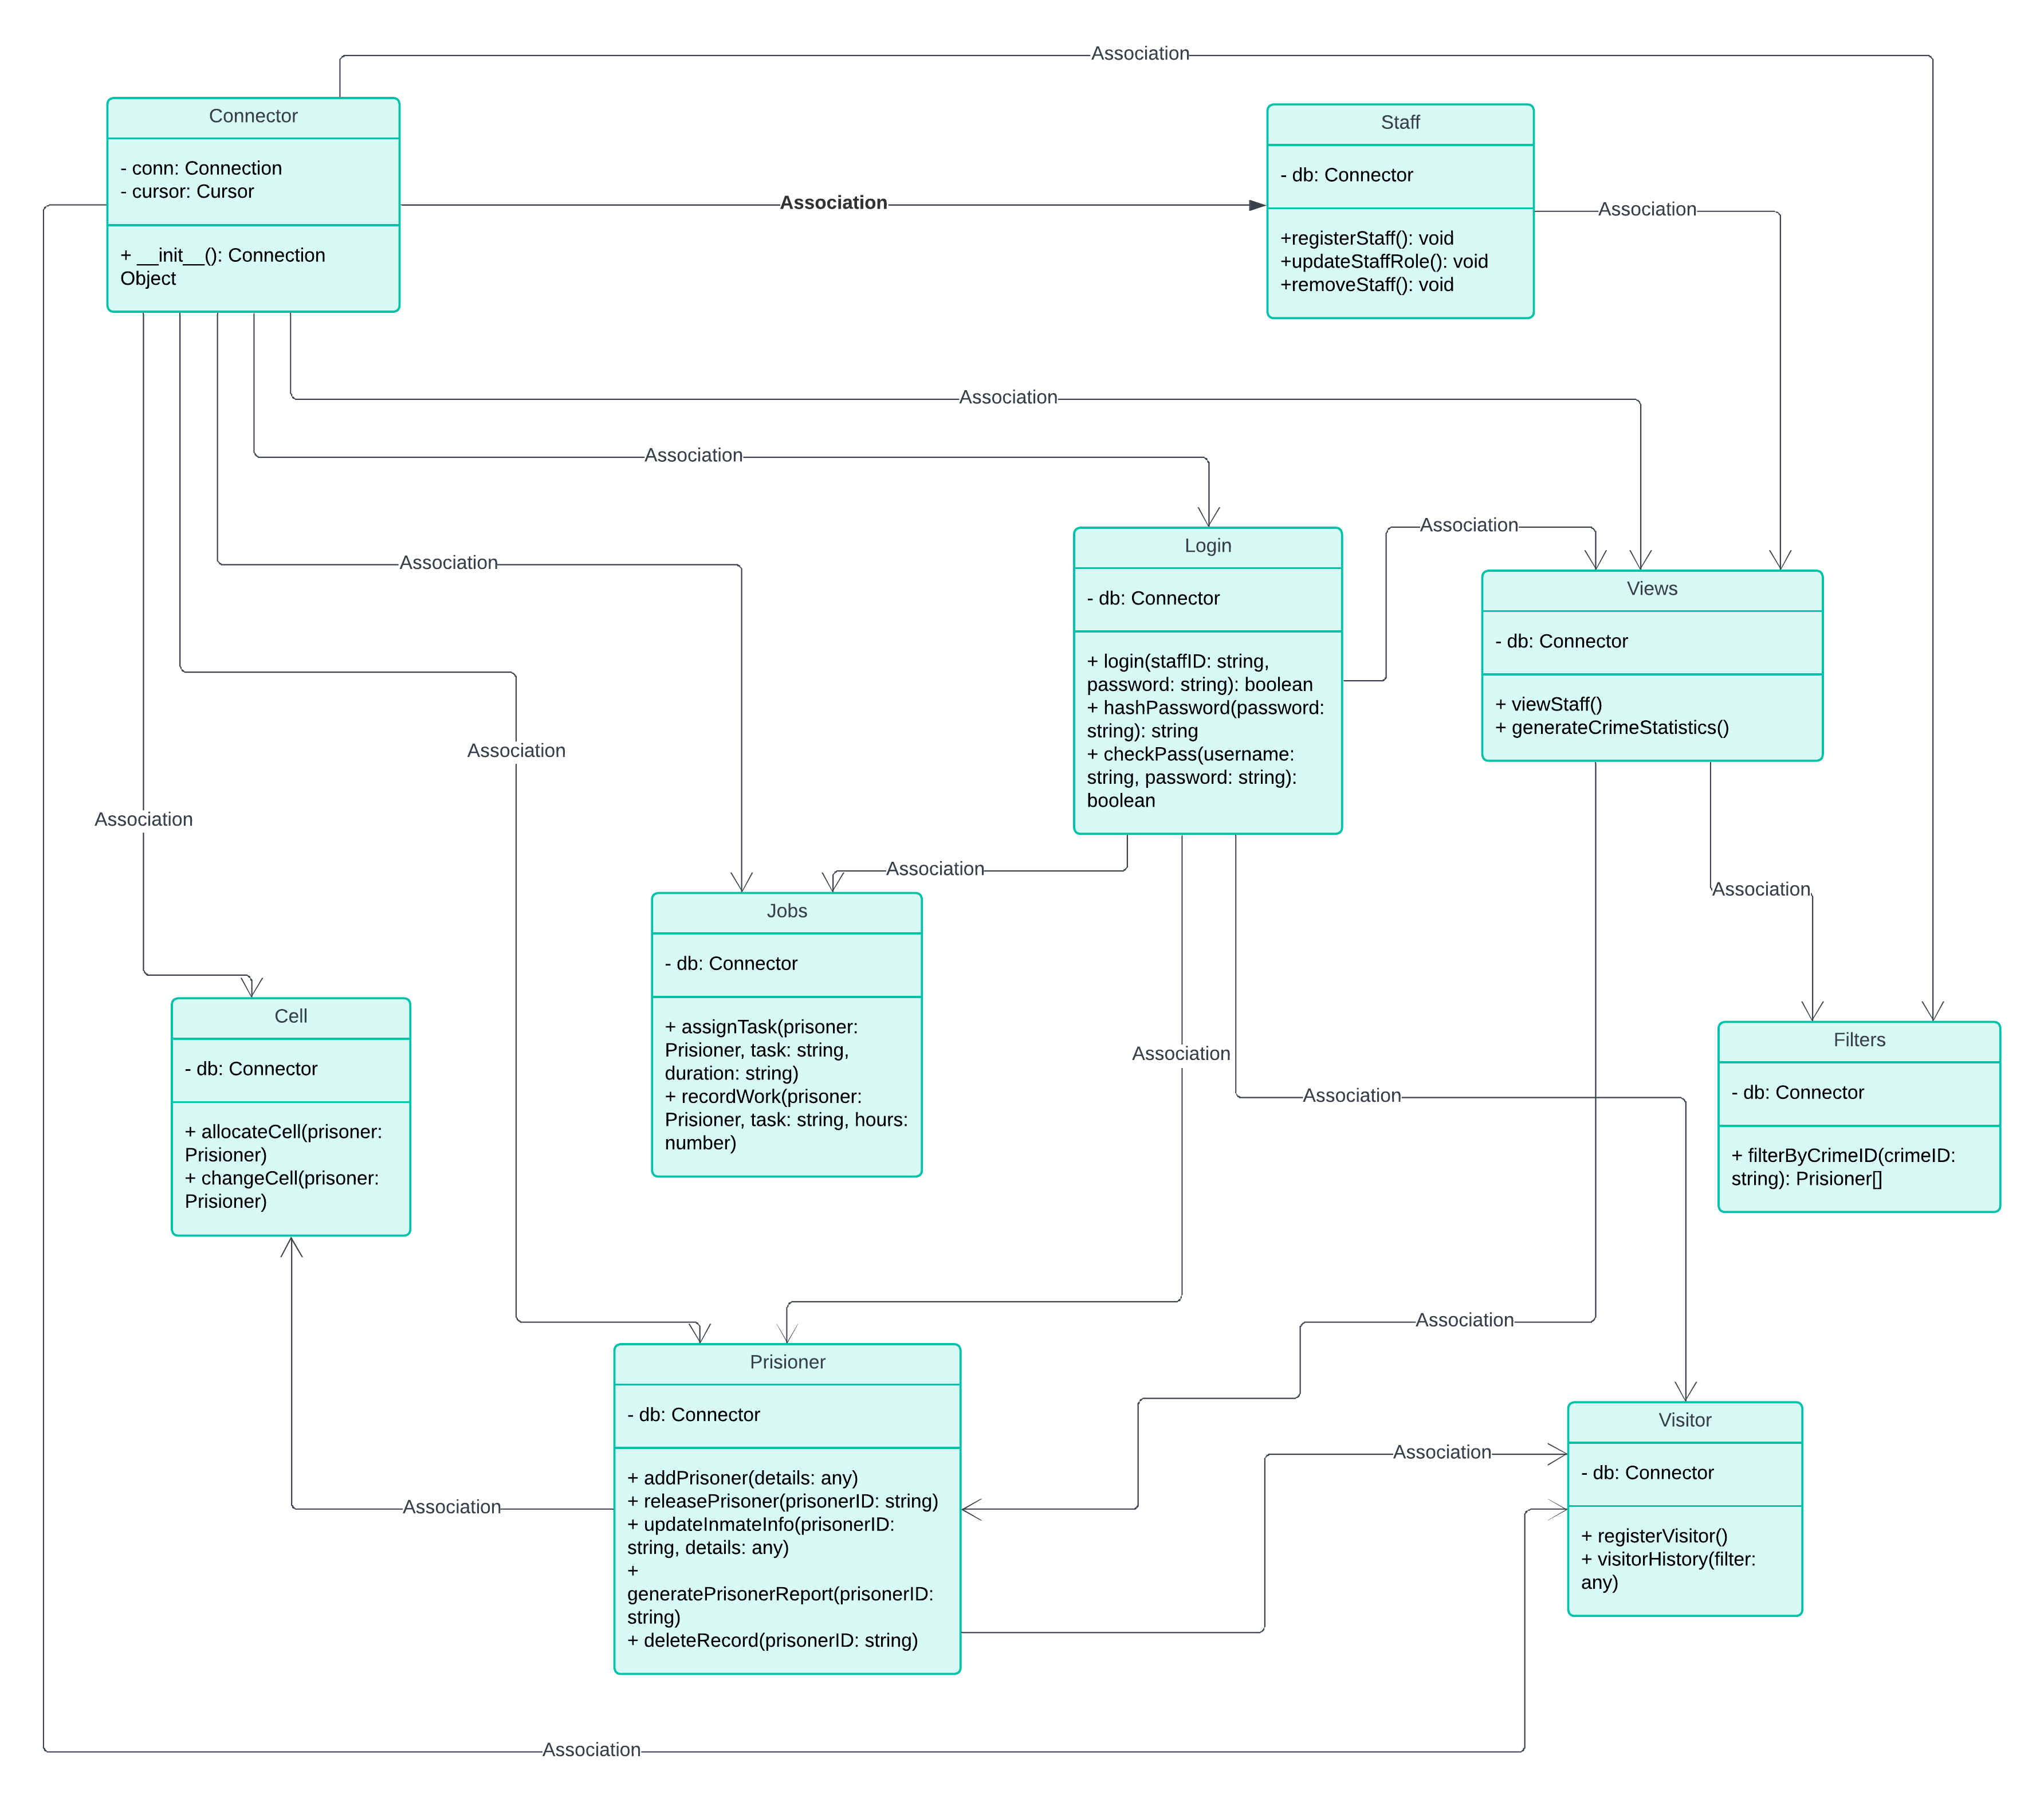
\includegraphics[angle=90, width=\textwidth, height=\textheight, keepaspectratio]{class3.png}
        \caption{Class Diagram}
        \label{fig:class}
    \end{figure}
    \newpage
    The following sequence diagram shows the sequence of operation of the system when a user interacts with it. The warden can use the various modules to manage different aspects of the prison such as staff and prisoner management.
    \begin{figure}[H]
        \centering
        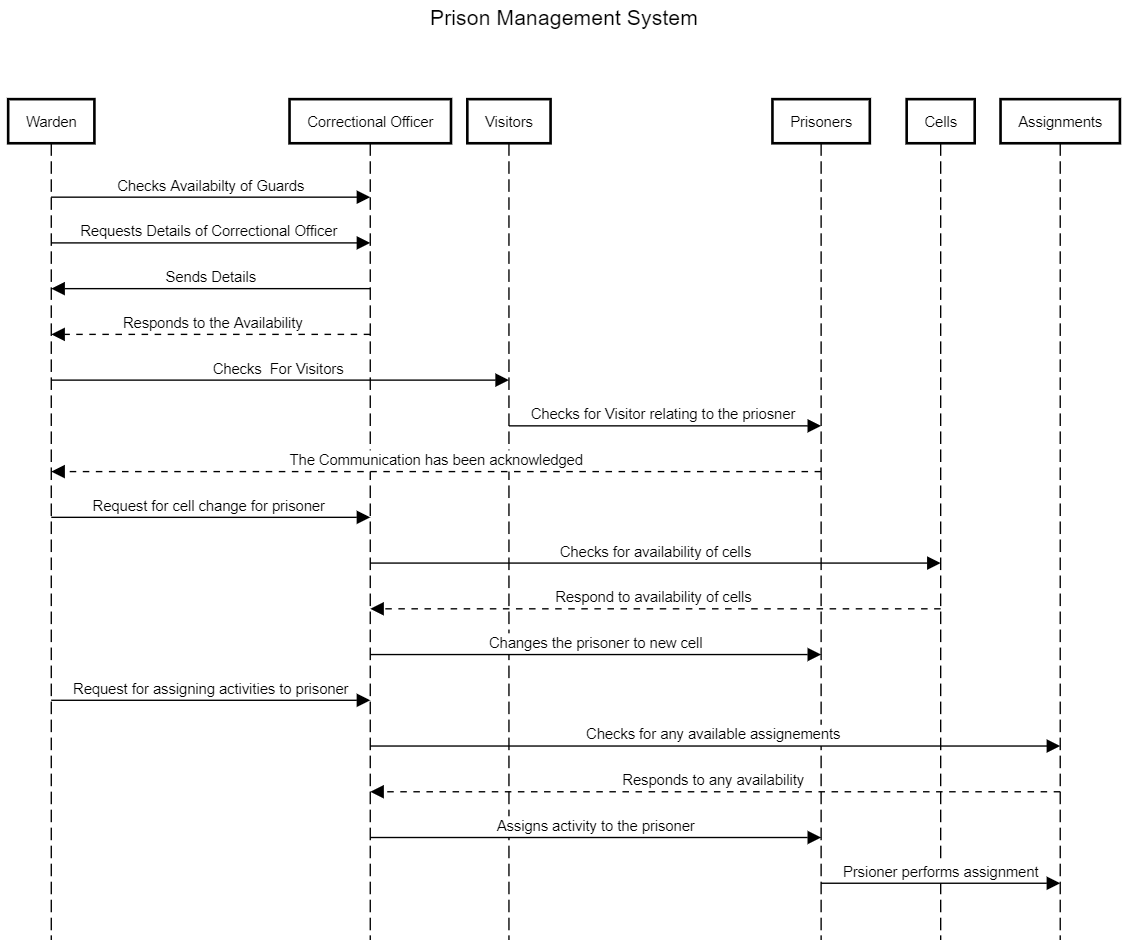
\includegraphics[scale=0.45, width=\textwidth]{sequence.png}
        \caption{Sequence Diagram}
        \label{fig:sequence}
    \end{figure}
    The Activity Diagram for the  PMS visually represents the flow of activities and actions within the system. It starts with the user arriving at the home page where they can log in. After providing correct credentials, the user is logged in and redirected to the dashboard where they can perform various actions related to the PMS. The user can view details regarding the prisoners, visitors, community service, cells, and staff and can add, remove, and modify the various details.
    \begin{figure}[H]
        \centering
        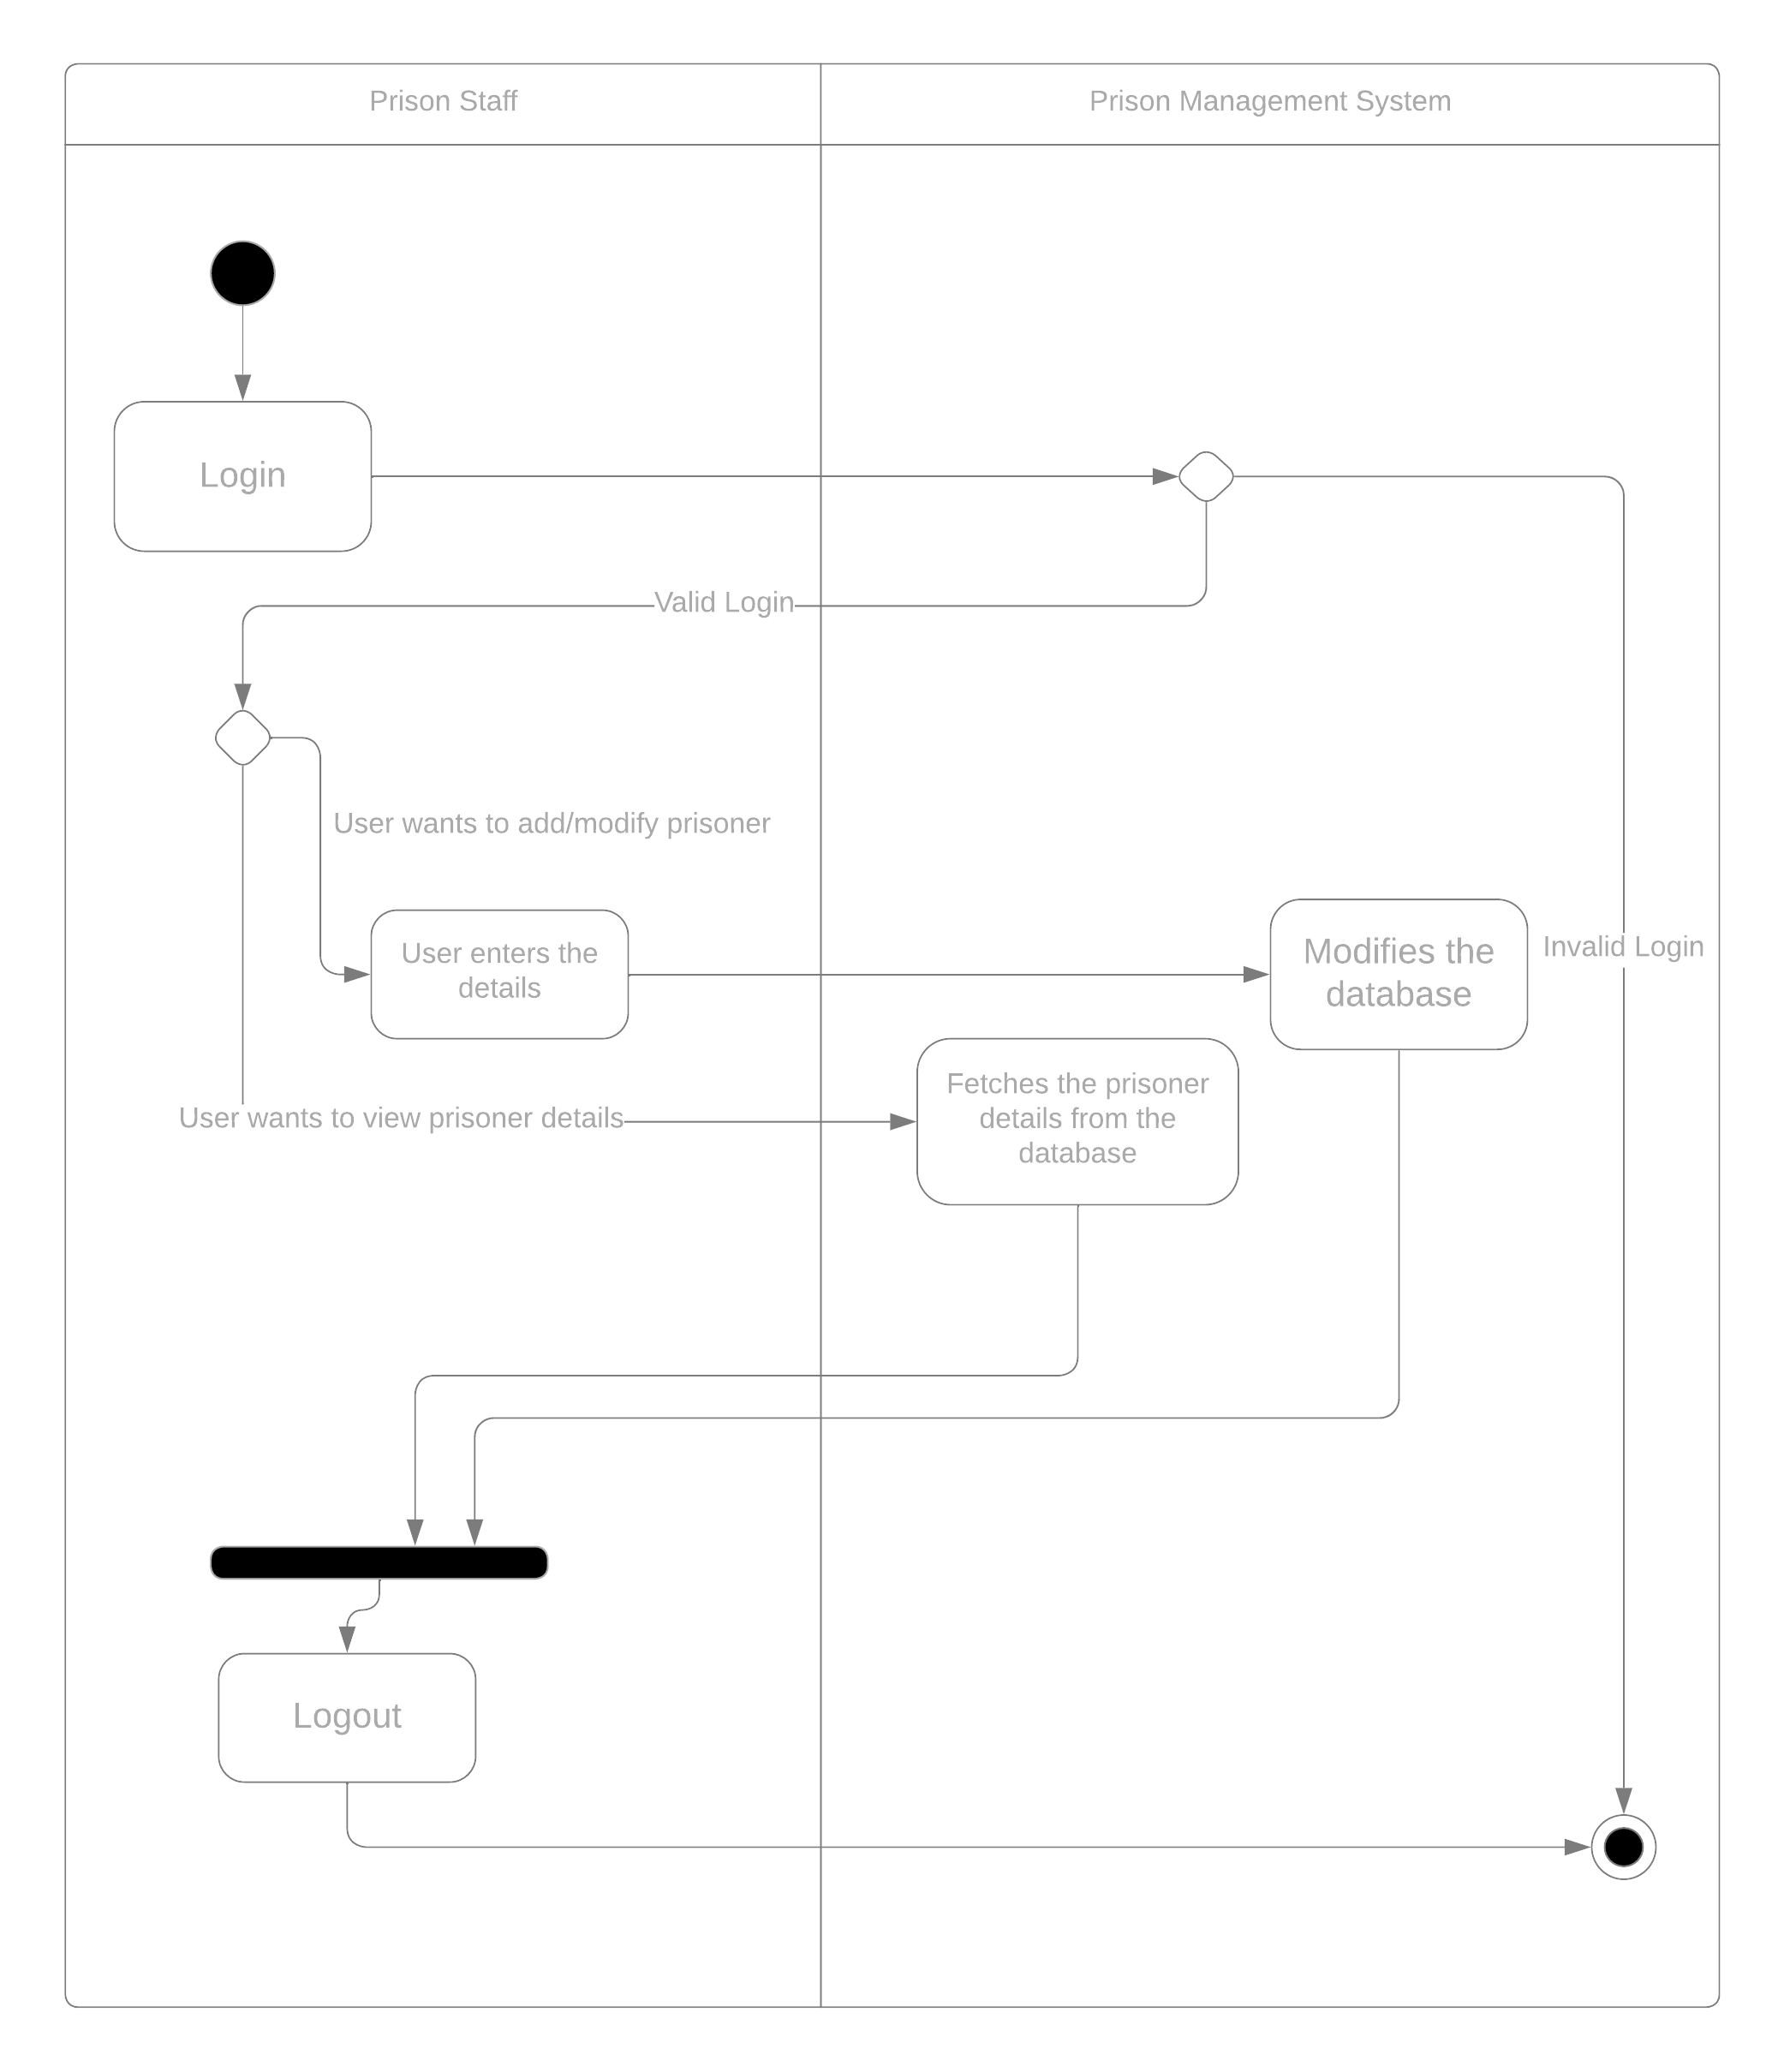
\includegraphics[scale=0.4, width=\textwidth]{activity.png}
        \caption{Activity Diagram}
        \label{fig:activity}
    \end{figure}
\subsection{User Interface}
    When the user opens the website, the landing page shows a form to login to the PMS. On successful login, the users are redirected to the dashboard. Here, they have the provision to view and modify various details regarding the prison. Upon choosing an option, they are shown the values in the table, along with buttons to add, delete or modify the various details.
    
\section{Hardware and Software Requirements}
\subsection{Hardware Requirements}
\begin{enumerate}
    \item Operating System: Windows 7 and above, Linux and macOS.
    \item Processor: 2 GHz processor or better.
    \item RAM: Minimum 4 GB RAM.
    \item Hard disk: Minimum 1 GB HDD Space.
    \item Internet Connection: Minimum 1 Mbps bandwidth.
\end{enumerate}    
\subsection{Software Requirements}
\begin{enumerate}
    \item \textbf{Programming Languages:} Python is used due to its extensive libraries and frameworks. JavaScript is used to create the Frontend using the ReactJS framework \cite{reactdocs}.

    \item \textbf{Libraries and Packages:} Hashlib is used to hash the passwords and MySQL Connector is used to connect with the database.
    
    \item \textbf{Integrated Development Environment (IDE):} IDE for coding, debugging, and testing. Common choices include Jupyter Notebooks, Visual Studio Code, or PyCharm.

    \item \textbf{Database Management System (DBMS):} To store and manage the grading data. MySQL is a popular relational database that was used for this project.
    
    \item \textbf{Web Framework:} Web Framework Flask \cite{flaskdocs} was used for Backend development.
    
    \item \textbf{Version Control:} Implement version control using Git to track changes in your codebase and collaborate with others.
\end{enumerate}
